%====================
% Nastaveni vlastnich stylu. 
%====================
\lstset{
tabsize = 4, 
showstringspaces = false, 
numbers = left, 
keywordstyle = \color{blue},
rulecolor = \color{black},
basicstyle = \small \ttfamily , 
breaklines = true,
numberstyle = \tiny,
xleftmargin=2em,
xrightmargin=0.5em,
frame=single,
framexleftmargin=1.5em
}
%====================
% Vlastní text BP
%====================
\chapter{Úvod}
\label{uvod}
V~době nepřeberného množství textových editorů a~integrovaných vývojových prostředí je třeba~zajistit komplexní podporu širokého množství programovacích jazyků. Taková podpora~zahrnuje například rozšířené funkce editorů jako je zvýrazňování syntaxe, dokončování kódu a~jiné.  Aby bylo možné implementaci těchto funkcí usnadnit, byl vyvinut \emph{Language Server Protocol}. \emph{Language Server Protocol} umožňuje zjednodušení celého procesu do implementace jednoho jazykového serveru (\emph{Language Server}) pro právě jeden programovací jazyk, který zajistí podporu daných funkcí za~užití volání vzdálené procedury (\emph{remote procedure call}). Pro implementaci na~straně klienta~je pak jen nutné zajistit komunikaci s~jazykovým serverem pro poskytnutí jazykové podpory. Hlavním cílem bakalářské práce je navrhnout a~implementovat jazykového klienta~pro integrované vývojové prostředí \emph{Apache NetBeans}.

\section{Motivace}
Již existující jazykový server vytvořený společností \emph{Red Hat} pro \emph{Apache Camel}~\cite{CamelLanguageServerGithub} aktuálně nabízí podporu pro integrovaná vývojová prostředí \emph{Eclipse, Microsoft Visual Studio Code, Eclipse Che} a~\emph{Atom}. Vytvoření jazykového klienta~pro komunitní vývojové prostředí \emph{Apache NetBeans} zajistí širší dostupnost pro uživatele. Zhotovení klienta~povede k~následnému zveřejnění v~\emph{Apache NetBeans Plugin Portalu} a~nasazení v~praxi.

\chapter{Přehled souvisejících technologií}
V~dnešní době jsou technologie neustále se rozvíjejícím prvkem každodenního života. Nové a~inovativní technologie se objevují každým dnem a~pomáhají řešit různé problémy. Účelem této kapitoly je popsat technologie související s~klientskou aplikací pro jazykový server \emph{Apache Camel}. Kapitola~se dále věnuje popisu samotného integračního rámce \emph{Apache Camel}.

\section{Language Server Protocol}
\label{lsp} 
\emph{Language Server Protocol} (neboli \emph{LSP})~\cite{lspgithub} je otevřený standardizovaný protokol pro komunikaci mezi textovým editorem či integrovaným vývojovým prostředím (\emph{IDE}) a~serverem poskytujícím podporu pro rozšíření vlastností editoru pro daný programovací jazyk. Protokol byl původně vyvíjen společností \emph{Microsoft} pro užití v~\emph{Microsoft Visual Studio Code}. V~roce 2016 společnost \emph{Microsoft} oznámila~spolupráci s~firmami \emph{Red Hat} a~\emph{Codenvy} za~účelem standardizace protokolu. 

Mezi typická rozšíření vývojových prostředí patří například zvýrazňování syntaxe, nápověda~a~dokončování kódu, formátování kódu, odkazování a~přechody na~definice či zpracování upozornění a~chyb.
Implementace těchto vlastností do jednotlivých textových editorů a~vývojových prostředí je náročná na~zdroje, zejména~na~čas. Použití různých aplikačních programových rozhraní (\emph{API}) v~jednotlivých prostředích znemožňuje snadné integrování totožných funkcí. Hlavní myšlenkou je standard, který přesouvá veškerou logiku daných funkcí na~stranu jazykového serveru. Ta~je následně z~editoru zpřístupněna~pomocí \emph{LSP} protokolu. 

\subsection{Princip funkce protokolu}
\label{lspPrincip}
\emph{LSP} je provozován jako separátní (samostatně běžící) proces, během kterého editor komunikuje s~jazykovým serverem za~použití bezstavového protokolu \emph{JSON-RPC}. Obrázek~\ref{editorLSPcommunicationScheme} znázorňuje komunikaci graficky.
Komunikace probíhá následovně:
\begin{enumerate}
    \item{Uživatel otevřel soubor ve svém editoru.
    \setlist{leftmargin=0mm} %odsazeni
    \begin{itemize}[label={}]
        \item{Editor upozorní jazykový server, že došlo k~otevření dokumentu pomocí notifikace \texttt{textDocument/didOpen}. Od tohoto okamžiku není obsah dokumentu pod správou souborového systému počítače, ale je uložen ve vnitřní paměti editoru, kde dochází k~synchronizaci mezi editorem a~jazykovým serverem za~užití \emph{LSP}.}
    \end{itemize}
    }

    \newpage
    \item{Uživatel provedl změnu.
    \setlist{leftmargin=0mm} %odsazeni
    \begin{itemize}[label={}]
        \item{Editor upozorní jazykový server pomocí notifikace \texttt{textDocument/didChange}. Jazykový server provede analýzu nově obdržených informací a~editoru odpovídá pomocí notifikace \texttt{textDocument/publishDiagnosis} obsahující diagnostiku včetně případných upozornění a~chyb.}
    \end{itemize}
    }
 
    \item{Uživatel vyžádal přechod na~definici (definující část) symbolu.
    \setlist{leftmargin=0mm} %odsazeni
    \begin{itemize}[label={}]
        \item{Editor odešle notifikaci \texttt{textDocument/definition}, která přijímá dva~parametry. Prvním parametrem je \texttt{documentURI}, nesoucí \emph{URI} odkazovaného dokumentu. Druhý parametr \texttt{position} udává konkrétní pozici definice uvnitř souboru odkazovaného v~\emph{URI}. Editor jako odpověď na~daný požadavek obdrží lokaci požadované definice.}
    \end{itemize}
    }
    
    \item{Uživatel zavřel dokument.
    \setlist{leftmargin=0mm} %odsazeni
    \begin{itemize}[label={}]
        \item{Notifikace \texttt{textDocument/didClose} je zaslána~z~editoru na~jazykový server. Ten je informován o~uzavření dokumentu a~tedy i o~tom, že není třeba~jej dále držet v~paměti. Na~zařízení se uloží poslední úpravy z~paměti do souborového systému.}
    \end{itemize}
    }
\end{enumerate}

\begin{figure}[hbt]
	\centering
        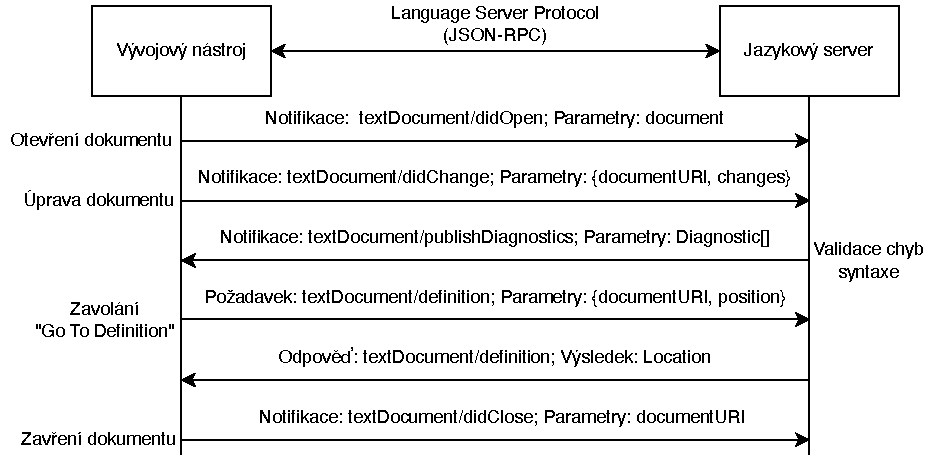
\includegraphics[width=1\columnwidth]{obrazky-figures/pdf/komunikace_editor_a_server.pdf}
	\caption{Grafické znázornění komunikace mezi editorem a~jazykovým serverem. Převzato z~\cite{MicrosoftLSPOverview}.}
	\label{editorLSPcommunicationScheme}
\end{figure}

\vspace{-10pt} % Pak se vleze na jednu stranu.
\subsection{Schopnosti protokolu}
\label{lspSchopnosti}
Ne každý jazykový server dokáže podporovat všechny funkce definované protokolem. \emph{LSP} proto poskytuje výčet podporovaných funkcí. Schopnost (\emph{Capability}) sdružuje sady podporovaných funkcí. Editor a~server si oznamují podporované funkce právě použitím capabilities. Např. server oznamuje, že dokáže zpracovat požadavek \texttt{textDocument/definition} (přechod na~definici), ale nedokáže zpracovat požadavek \texttt{workspace/symbol} (vyhledávání symbolů). Editor tak ví, které požadavky má smysl na~server odesílat ke zpracování a~které ne. Stejně tak je možné, že editor oznámí své schopnosti poskytovat notifikace typu \texttt{about to save}. Server tak může zpracovávat kód průběžně, ještě než je uložen a~požadavek odeslán. 

\subsection{Současná práce s~více jazyky}
\label{lspPraceSViceJazyky}
Když uživatel pracuje zároveň s~více jazyky, editor naváže komunikaci s~jazykovým serverem pro každý jazyk zvlášť. Obrázek~\ref{multipleLanguageCommunication} graficky znázorňuje proces komunikace s~více jazykovými servery.

\begin{figure}[hbt]
	\centering
        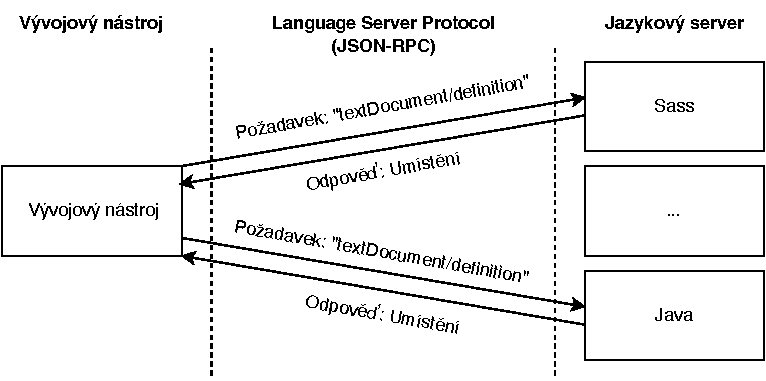
\includegraphics[width=1\columnwidth]{obrazky-figures/pdf/komunikacepripracisvicejazyky.pdf}
	\caption{Schéma~komunikace editoru a~serveru při práci s~více jazyky. Převzato z~\cite{MicrosoftLSPOverview}.}
	\label{multipleLanguageCommunication}
\end{figure}


\subsection{Specifikace protokolu}
\label{lspSpecifikace}
Základní protokol je tvořen hlavičkou a~obsahem. Protokol je podobný \emph{HTTP}. Hlavička a~obsah jsou odděleny pomocí \texttt{\symbol{92}r\symbol{92}n}. V~této práci bude použita~verze protokolu 3.17, která je poslední dostupnou (kontrolováno dne 15.04.2023).

\subsubsection{Hlavičková část}
Skládá se z~dvou hlavičkových polí. Každé pole je složeno ze jména~a~hodnoty oddělené \texttt{': '} (dvojtečka~následovaná mezerou). Struktura~hlavičkových polí vyhovuje \emph{HTTP} sémantice. Každé pole je ukončeno pomocí \texttt{\symbol{92}r\symbol{92}n}. Poslední pole v~hlavičce je povinné. To znamená, že obsahové části zprávy vždy předcházejí dvě sekvence ukončovacích znaků \texttt{\symbol{92}r\symbol{92}n}. Tabulka~\ref{podporovaneHlavicky} popisuje současně podporovaná pole.

\begin{table}[hbt]
\centering
\begin{tabular}{|l|c|c|}
\hline
Typ hlavičky & Datový typ & Popis \\ \hline
Content-Length & číslo & Délka~obsahu v~bytech. Toto pole je povinné. \\ \hline
Content-Type & řetězec & Samotný obsah. Implicitně nastaven na~\\ 
& & \texttt{application/vscode-jsonrpc; charset=utf8}. \\ \hline
\end{tabular}
\caption{\label{tab:SoucasnePodporovanaHlavickovaPole}Výčet současně podporovaných hlavičkových polí.}
\label{podporovaneHlavicky}
\end{table}

\subsubsection{Obsahová část}
Obsahuje vlastní obsah zprávy. Zpráva~používá protokol \emph{JSON-RPC}, aby popsala~objekt, kterým může být požadavek, odpověď či notifikace. Více viz kapitola~\ref{jsonrpc} věnující se \emph{JSON-RPC}. Kódování obsahové části je definováno v~poli \texttt{Content-Type}. Implicitně je využíváno kódování \texttt{utf–8}, které je jediné podporované v~\emph{LSP}. V~případě, že klient nebo server obdrží požadavek s~rozdílným kódováním, končí požadavek chybou. Starší verze používaly chybné označení -- \texttt{utf8}. Správně implementovaný klient i server by měly toto označení kódování považovat za~totožné s~\texttt{utf-8}.

\begin{lstlisting}[language=JAVA, caption=Ukázka~obsahu zprávy.]
Content-Length: ...\r\n
\r\n
{
	"jsonrpc": "2.0",
	"id": 1,
	"method": "textDocument/completion",
	"params": {
		...
	}
}
\end{lstlisting}

\subsection{Architektura~protokolu}
\label{jsonrpcArchitektura}
Architekturu lze popsat několika~základními prvky sloužícími pro komunikaci mezi editorem a~jazykovým serverem. Prvky jsou následující:

\begin{itemize}
    \item{\textbf{Language Client} -- Zprostředkovává komunikaci editoru a~jazykového serveru.
    }
    \item{\textbf{Language Server} -- Zpracovává požadavky klienta, komunikuje s~editorem, využívá svých vlastností pro adekvátní odpověď klientovi.
    }
    \item{\textbf{Language Server Protocol} -- Samotný protokol sloužící pro přenos dat. Pro přenos využívá \textit{JSON-RPC}.
    }
\end{itemize}

\section{JSON-RPC}
\label{jsonrpc}
Je bezstavový protokol využívající vzdáleného volání procedur (\emph{remote procedure call}, neboli \emph{RPC}). To znamená, že požadovaná procedura~je vykonána~v~jiném adresovém prostoru, ale zároveň vývojář nemusí explicitně řešit implementaci vzdálené integrace. Vytváří stejný kód bez ohledu na~to, zda~je daná interakce obsluhována~lokálně nebo vzdáleně. Samotný protokol \emph{JSON-RPC} byl navržen tak, aby byl co nejjednodušší. Obsahuje tedy pouze několik datových typů a~operací nad nimi. 

V~rámci práce budeme pracovat s~verzí protokolu \emph{JSON-RPC 2.0}, která je poslední dostupnou (kontrolováno dne 15.04.2023),

\newpage
\subsection{Vlastnosti JSON-RPC}
\label{jsonrpcVlastnosti}
Protokol podporuje odesílání požadavků, odpovědi, události a~chyby. Každý z~těchto datových typů je pojímán jako objekt. Klient (editor) obvykle požaduje pouze jednu metodu ze vzdáleného serveru. Více vstupních parametrů je možné předávat serveru jako pole (array). Vzdálená metoda~může podobným způsobem vracet více výstupních dat.\footnote{Není dostupné ve starších verzích.} Objekty je možné serializovat (skládat za~sebe) tak, jak umožňuje protokol \emph{JSON}. 

\subsection{Objekty v~JSON-RPC}

\subsubsection{Požadavek}
Volání~ specifické~ metody~ poskytnuté~ vzdáleným~ serverem. Objekt~ obsahuje~ parametr \texttt{jsonrpc}, který určuje verzi \textit{JSON-RPC} protokolu. Dále může obsahovat až tři další členy:

\begin{itemize}
    \item{\textbf{method} -- Řetězec obsahující jméno metody, která má být vyvolána. Nesmí začínat předponou \texttt{rpc}. Takové metody jsou rezervovány pro vnitřní užití v~rámci protokolu. 
    }
    \item{\textbf{params} -- Objekt nebo pole s~hodnotami, které jsou předávány volané metodě. Pole musí obsahovat prvky v~pořadí, které je očekávané druhou stranou. Objekt musí obsahovat přesný název, který očekává druhá strana. Použití tohoto parametru není vyžadováno.
    }
    \item{\textbf{id} -- Řetězec nebo celé číslo užívané k~identifikaci a~provázání odpovědi a~požadavku. Není-li očekávaná žádná odpověď, lze tento parametr vynechat.
    }
\end{itemize}

\subsubsection{Odpověď}
Reakce na~obdržené volání specifické metody. Objekt obsahuje parametr \texttt{jsonrpc}, který určuje verzi \emph{JSON-RPC} protokolu. Dále může obsahovat až tři další členy:

\begin{itemize}
    \item{\textbf{result} -- Data~odpovídají návratové hodnotě vyvolané metodou. V~případě úspěšného vykonání je formátován jako \emph{JSON} objekt. V~případě, že během zpracování došlo k~chybě, musí tento člen zůstat nepoužitý.
    }
    \item{\textbf{error} -- Návratová hodnota~je objekt příslušné chyby. Viz tabulka~\ref{jsonrpcerrorcodes}. Dojde-li během zpracování požadavku k~chybě, musí být tento člen přítomný. Nedojde-li k~chybě během zpracování, není přítomnost členu nutná.
    }
    \item{\textbf{id} -- Hodnota~odpovídající \texttt{id} obdrženého požadavku.
    }
\end{itemize}

\subsubsection{Notifikace}
Z~hlediska~protokolu se jedná o~objekt požadavku, jeho parametr \texttt{id} je ale vždy \texttt{NULL}. Na~tento typ objektu není očekávaná odpověď, není tedy přítomnost \texttt{id} vyžadována.

\subsubsection{Chyba}
Objekt chyby je struktura~obsahující informace o~chybě, která se vyskytla~při zpracování požadavku. Tento objekt se používá k~informování klienta~o~chybě, která se vyskytla~v~LSP serveru, aby mohl klient provést nápravné kroky.

\begin{itemize}
    \item{\textbf{code} -- Obsahuje celočíselnou hodnotu nesoucí hodnotu příslušné chyby. Tabulka~\ref{jsonrpcerrorcodes} obsahuje výčet jednotlivých chybových kódů.}
    \item{\textbf{message} -- Řetězec obsahující chybové hlášení.}
    \item{\textbf{data} -- Podrobnější popis chyby. Parametr není povinný.}
\end{itemize}

\begin{table}[hbt]
\centering
\begin{tabular}{|l|c|c|}
\hline
kód & zpráva~& význam \\\hline
-32700 & Chyba~syntaktické analýzy. & Server obdržel neplatný \emph{JSON}. Chyba~ \\ 
& & nastala~během syntaktické \\ 
& & analýzy na~serveru. \\\hline
-32600 & Neplatný požadavek.  & Odeslaný \emph{JSON} není platným \\ 
& & objektem  Požadavku.\\\hline
-32601 & Metoda~nebyla~nalezena. & Požadovaná metoda~neexistuje \\
& & nebo není dostupná. \\\hline
-32602 & Neplatný parametr.  & Neplatný parametr požadované \\
& & metody. \\\hline
-32603 & Vnitřní chyba. & Vnitřní chyba~protokolu \emph{JSON-RPC}. \\\hline
-320xx & Chyba~serveru. & Kódy vyhrazené pro chyby \\
& & definované implementovaným serverem.\\\hline
\end{tabular}
\caption{\label{tab:chyboveKodyJson}Přehled chybových kódů protokolu \emph{JSON-RPC}.}
\label{jsonrpcerrorcodes}
\end{table}

\subsection{Hromadné volání}
\label{jsnorpcHromadnevolani}
Protokol umožňuje hromadné volání metod. V~takovém případě klient odesílá pole naplněné objekty požadavků. Server dané požadavky zpracuje, odpovědi plní do pole a~po zpracování všech požadavků vrací pole odpovědí. Server požadavky může zpracovat v~libovolném pořadí. To znamená, že pole odpovědí je naplněno také v~libovolném pořadí. Klient musí jednotlivé odpovědi propojit na~základě \texttt{id} požadavku. 

V~případě že dojde k~chybě zpracování během hromadného volání, např. že požadavek není rozpoznán jako validní \emph{JSON} nebo pole s~alespoň jednou hodnotou, odpověď musí být pouze jeden objekt odpovědi. Pokud není server schopen zpracovat ani jeden z~požadavků a~pole odpovědí je tedy prázdné, nesmí toto pole server vrátit. V~takovém případě není navráceno nic.

\section{Apache Camel}
\label{camel}
\emph{Apache Camel} je open-source integrační rámec (\emph{framework}) vytvořený v~jazyce \emph{Java}. Je založený na~\emph{Enterprise Integration Patterns} popsaných v~knize od Gregora~Hohpe a~Bobbyho Woolfa~\cite{Hohpe2004}. Základní koncept je tvořen integrací a~interakcemi mezi různými aplikacemi, pro které \emph{Camel} poskytuje trasování (routing), transformování a~monitorování. \emph{Camel} narozdíl od \emph{ESB} (\emph{Enterprise Service Bus}) nepodporuje kontejnery nebo spolehlivé zprávové sběrnice (\emph{message bus}). Lze na~jeho základě ale vytvořit kompletní integrační platformy jako je například \emph{JBoss Fuse}~\cite{JBossFuse} nebo \emph{Apache ServiceMix}~\cite{ApacheServiceMix}. \emph{Camel} užívá modulární architekturu, která umožňuje implementaci a~použití zásuvných modulů pro podporu nových protokolů. Díky použití tohoto designu je architektura~\emph{Apache Camel} rychlá a~snadno rozšiřitelná pro vývojáře.

\subsection{Vlastnosti}
\label{camelVlastnosti}
\emph{Camel} k~zápisu integračních cest užívá stanovené konvence, které jsou dány doménově specifickým jazykem (\emph{Domain Specific Language - DSL}) v~deklarativní podobě. Nejčastější formou zápisu dané cesty je užití programovacího jazyka~\emph{Java}, který umožňuje za~použití frameworků \emph{Spring}~\cite{SpringFramework} (ukázka~viz výpis~\ref{lst:apachecamel-springdsl-ukazka}), \emph{Blueprint}~\cite{BlueprintFramework} nebo \emph{Scala}~\cite{ScalaFramewoek} definovat konfigurační soubory \emph{XML}. Dále je možné použít definici pomocí běžného kódu \emph{Java}~(\emph{Java~DSL}~\cite{JavaDSLFramework}) bez nutnosti použití konfiguračních souborů. Oba~druhy zápisu jsou téměř totožné. \emph{Blueprint} se typicky nasazuje v~rámci \emph{OSGi} (\emph{Open Services Gateway initiative})~\cite{OSGi}.

\begin{lstlisting}[language=XML, label={lst:apachecamel-springdsl-ukazka}, caption=Ukázka~syntaxe pro \emph{Spring DSL}.]
<routes xmlns="http://camel.apache.org/schema/spring">
    <route>
        <from uri="timer:tick"/>
        <setBody>
            <constant>Hello World!</constant>
         </setBody>
        <to uri="log:info"/>
    </route>
</routes>
\end{lstlisting}

\subsection{Trasování}
\label{camelTrasovani}
Základní vlastností \emph{Apache Camel} je jeho trasovací a~zprostředkovací engine (\emph{routing and mediation engine}). Trasovací engine přesouvá data~z~jedné lokace do jiné. Při tomto přesunu využívá nakonfigurovaných cest. Uživatel si může pro svoje trasování nadefinovat vlastní pravidla, přidávat metody pro zpracování a~modifikaci dat a~data~filtrovat. Na~konci cesty je také potřeba~zvolit cílovou lokalitu, kam budou umístěna~výstupní data.

\subsection{Transformace}
\label{camelTransformace}
Transformace (přeměna~vstupní informace na~výstupní) přes definovanou cestu probíhá po objektech zprávy. 
 
\subsubsection{Objekt Zpráva}
\label{camelObjZprava}
Objekt \emph{Zpráva}~(Message) [\texttt{org.apache.camel.Message}] reprezentuje data, která jsou používána~systémem ke vzájemné komunikaci. Komunikace probíhá od odesílatele k~příjemci. Objekt \emph{Zprávy} se skládá z~hlavičky, těla~zprávy a~nepovinných příloh. Všechny \emph{Zprávy} jsou identifikovány unikátním identifikátorem. Tvar identifikátoru je definován konvencí protokolu. V~případě, že protokol tvar identifikátoru nedefinuje, je užita~výchozí konvence integračního rámce. 

Hlavička~\emph{Zprávy} je obdobná hlavičce protokolu \emph{HTTP}. Obsahuje informace o~odesílateli, kódování, typ obsahu a~autentizační parametry. Tělo reprezentuje obsah samotné zprávy. Typicky se jedná o~\emph{Java}~objekt, zpráva~může uložit jakýkoliv typ obsahu, pouze by měla~být zajištěna~schopnost příjemce danou zprávu akceptovat.

\subsubsection{Objekt Výměna}
\label{camelObjVymena}
Objekt \emph{Výměny} je definován jako kontejner zapouzdřující objekt \emph{Zprávy} během jeho cesty. Mezi objektem \emph{Výměny} a~systémem probíhá množství interakcí. Grafické znázornění objektu je popsáno obrázkem~\ref{camelObjVymenaObr}.
Objekt obsahuje: 

\begin{itemize}
    \item \textbf{ID výměny} (\emph{Exchange ID}) -- Unikátní identifikátor dané výměny, může být explicitně daný, jinak je automaticky generovaný rámcem \emph{Apache Camel}.
    \item \textbf{Message Exchange Pattern} (\emph{MEP}) -- Definuje styl zprávy.
    \item \textbf{Výjimka}~(\emph{Exception}) -- Pro případ že by během cesty nastala~chyba.
    \item \textbf{Vlastnosti} (\emph{Properties}) -- Obdoba~hlavičky v~objektu Zprávy, vlastnosti jsou ale narozdíl od hlavičky neměnné po celou dobu trvání výměny.
    \item \textbf{Vstupní zpráva}~-- Povinná vstupní zpráva~obsahující požadavek.
    \item \textbf{Výstupní zpráva}~-- Nepovinná zpráva~obsahující odpověď (pouze pro \emph{Message Exchange Pattern} typu \emph{InOut}).
\end{itemize}

\begin{figure}[hbt]
	\centering
        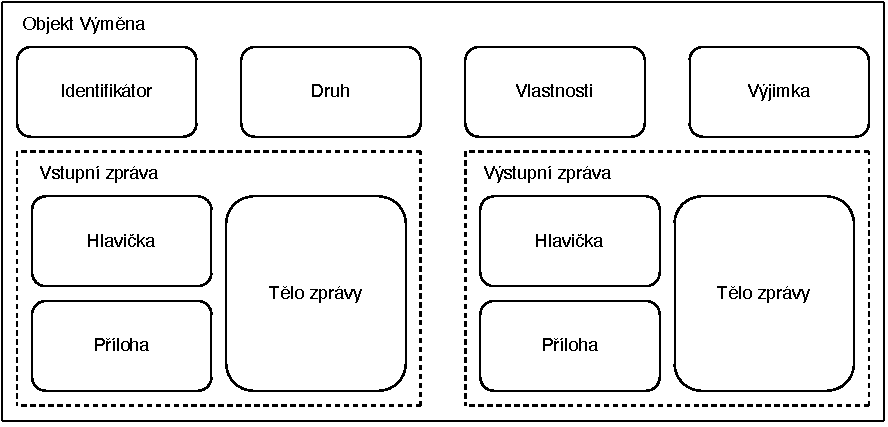
\includegraphics[width=1\columnwidth]{obrazky-figures/pdf/objektvymena.pdf}
	\caption{Znázornění objektu \emph{Výměny} a~jeho komponent.}
	\label{camelObjVymenaObr}
\end{figure}

\subsection{Architektura}
\label{camelArchitektura}
Architektura~\emph{Apache Camel} je založena~na~\emph{Camel Context}, který propojuje prvky architektury běhového systému.

\subsubsection{Camel Context}
Obdoba~kontejneru určená pro běhové prostředí (\emph{runtime}) systému \emph{Camel}. Kontext udržuje vše pohromadě a~spravuje následující služby během spuštěného běhového prostředí (graficky viz obrázek~\ref{camelcontext}):

\begin{itemize}
    \item \textbf{Cesty} (\emph{Routes}) -- nadefinované cesty mezi komponenty přidané do kontextu.
    \item \textbf{Cíle} (\emph{Endpoints}) -- Cíle jednotlivých cest vytvořených v~kontextu.
    \item \textbf{Komponenty} (\emph{Components}) -- Komponenty používané aplikacemi.
    \item \textbf{Typové převaděče} (\emph{Type Converters}) -- Možné změny datového typu načtené kontextem.
    \item \textbf{Datové formáty} (\emph{Data~formats}) -- Datové formáty načtené do kontextu.
    \item \textbf{Jazyky} (\emph{Languages}) -- \emph{Camel} podporuje různé jazyky použité ve výrazech, ty jsou načteny do kontextu. 
    \item \textbf{Registry} (\emph{Registers}) -- Implicitně je užitý \emph{Java~Naming and Directory Interface}~\cite{JNDI}, v~případě specifických požadavků technologie může být použit i jiný. 
\end{itemize}

\begin{figure}[hbt]
	\centering
        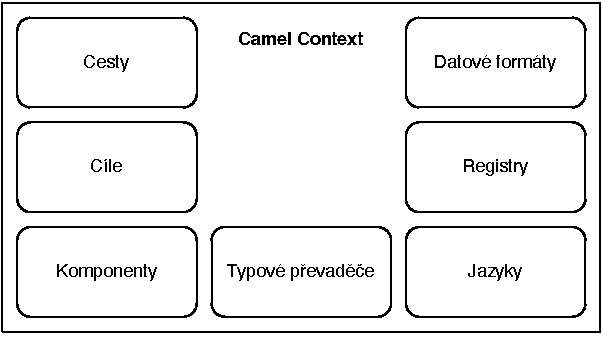
\includegraphics[width=0.75\columnwidth]{obrazky-figures/pdf/CamelContext.pdf}
	\caption{Jednotlivé prvky architektury, ze kterých je složený rámec \emph{Camel Context.}}
	\label{camelcontext}
\end{figure}

\subsection{Komponenty}
\label{camelKomponenty}
Jedním z~klíčových prvků \emph{Apache Camel} jsou komponenty. Komponenty v~\emph{Apache Camel} jsou moduly reprezentující systémy a protokoly, které lze integrovat dohromady. Každá komponenta~má specifické rozhraní pro komunikaci s~daným systémem a~umožňuje snadné propojení s~\emph{Apache Camel}. Komponenty mohou být použity jak pro odesílání, tak pro příjem zpráv. Každá komponenta~má svůj vlastní konfigurační soubor, který umožňuje nastavit vlastnosti pro daný systém. Například konfigurace komponenty pro práci s~databázemi umožňuje nastavit připojení k~databázi, \emph{SQL} dotazy a~další vlastnosti. V~současné době \emph{Apache Camel} podporuje více než 300 různých komponent.

Komponenty v~\emph{Apache Camel} lze použít pro vytváření integračních cest, které umožňují propojovat různé systémy a~aplikace. Jednotlivé cesty jsou tvořeny soubory komponent. Tyto cesty lze vytvářet pomocí konfiguračních souborů nebo v~kódu.

\subsection{Katalogy komponent}
\label{camelKatalogyKomponent}
Katalogy komponent v~\emph{Apache Camel} jsou soubory, které obsahují seznam komponent, které jsou dostupné pro použití. Tyto soubory jsou obvykle ve formátu \emph{XML} nebo \emph{JSON} a~obsahují informace o~každé komponentě. Mezi tyto informace patří například název, třída, verze a~další. Katalogy komponent jsou užitečné pro vývojáře, kteří chtějí použít \emph{Apache Camel} pro integraci s~konkrétním systémem. Díky tomu je možné provést snadnou instalaci a~konfiguraci potřebných komponent. Katalogy komponent jsou součástí \emph{Apache Camel} a~jsou distribuovány společně s~ním. Existují také externí katalogy komponent, které obsahují komponenty vyvinuté třetími stranami a~které lze použít s~\emph{Apache Camel}. Katalogy se mezi jednotlivými verzemi \emph{Apache Camel} můžou lišit.

\subsection{Běhová prostředí}
\label{camelBehovaProstredi}
Běhové prostředí \emph{Apache Camel} je softwarová komponenta~umožňující běh integračních cest a~řešení. Existuje mnoho různých poskytovatelů běhového prostředí pro \emph{Apache Camel}. Vzájemně se liší svými vlastnostmi a~použitím. Díky tomu lze optimalizovat běh \emph{Camel} aplikací pro konkrétní použití, prostředí a~scénáře. Nejpoužívanější běhová prostředí jsou:

\subsubsection{Spring Boot}
\emph{Spring Boot} je běhové prostředí, které je založeno na~\emph{Spring Frameworku}~\cite{SpringFramework}. Prostředí poskytuje všechny výhody a~funkce \emph{Spring Frameworku} a~umožňuje snadnou integraci s~jinými \emph{Spring} projekty. Jeho konfigurace je snadná, lze k~tomu použít \emph{Spring XML} nebo \emph{Java}~konfigurace. Běhové prostředí \emph{Spring Boot} je velmi flexibilní a~vhodné pro větší a~složitější projekty.

\subsubsection{Karaf}
\emph{Karaf} je běhové prostředí, které je založeno na~\emph{Apache Karaf}~\cite{ApacheKaraf}. \emph{Karaf} využívá \emph{OSGi}~\cite{OSGi} kontejnerů a~umožňuje snadnou správu modulů a~závislostí v~běhu aplikace. Jeho architektura~je modulární. V~rámci běhového prostředí jsou integrovány další technologie a~frameworky jako například \emph{Apache CXF}~\cite{ApacheCXF} nebo \emph{Apache ActiveMQ}~\cite{ApacheActiveMQ}. Běhové prostředí \emph{Karaf} je vhodné pro velké a~složité projekty, kde je potřeba~spravovat mnoho modulů a~závislostí.

\subsubsection{Quarkus}
\emph{Quarkus} je běhové prostředí založené na~open-source frameworku pro kontejnerizované mikroslužby. Jednou z~nejvýraznějších vlastností běhového prostředí \emph{Quarkus} je jeho rychlost a~nízká paměťová  náročnost, což umožňuje běh \emph{Camel} aplikací v~malých kontejnerech a~nízkou latenci. Dále umožňuje snadnou kombinaci různých technologií v~jedné aplikaci a~poskytuje vývojářům mnoho možností pro vytváření moderních cloudových a~bezserverových aplikací. Běhové prostředí \emph{Quarkus} podporuje různá prostředí, jako jsou \emph{Kubernetes}~\cite{Kubernetes}, nebo \emph{OpenShift}~\cite{OpenShift}. Běhové prostředí je vhodné pro vytváření efektivních, škálovatelných a~výkonných mikroslužeb, které jsou nasazeny v~kontejnerech.

\subsection{Apache Kafka}
\label{camelApacheKafka}
\emph{Apache Kafka}~je open-source streamovací platforma~navržená pro zpracování a~ukládání velkého množství dat v~reálném čase. \emph{Kafka}~se zaměřuje na~vysokou spolehlivost, škálovatelnost a~nízkou latenci a~je vhodná pro zpracování dat z~různých zdrojů, jako jsou například senzory, aplikace, webové stránky a~další. \emph{Kafka}~se často využívá pro zpracování velkých objemů dat v~aplikacích pracujících v~reálném čase. \emph{Kafka}~používá \emph{publish-subscribe} vzorec, kde producenti zapisují data~do \emph{topiců}\footnote{Topic je kanál pro ukládání a~přenášení zpráv, které jsou organizovány do oddělených a~nezávislých toků dat.} a~konzumenti je odebírají k~dalšímu zpracování.

\section{Jazykový server pro Apache Camel}
\label{jazykovyServerApacheCamel}
Implementace jazykového serveru pro \emph{Apache Camel} byla~vytvořená společností \emph{Red Hat} za~účelem poskytnutí jazykové podpory. Jedná se o~open-source projekt, jehož zdrojový kód je volně dostupný na~\emph{GitHub} repozitáři~\cite{CamelLanguageServerGithub}. Jazykový server je implementovaný v~jazyce \emph{Java}, využívá knihoven \emph{LSP4J} a~\emph{LSP4E} a~jeho provozování je nezávislé na~cílové platformě. 

Poslední dostupnou verzí ke dni 16.4.2023 je verze \texttt{1.9.1}. Vytvořený jazykový klient bude podporovat všechny současně podporované funkční vlastnosti. Mezi ty patří:
\begin{itemize}
    \item Dokončování kódu pro jednotné identifikátory zdroje (\emph{URI}) \emph{Camel}. To zahrnuje dokončování \emph{Camel} komponent, atributů a~jejich hodnot.
    \item Zobrazování dokumentace pro jednotlivé \emph{Camel} komponenty. 
    \item Diagnostika~a~validace jednotných identifikátorů zdroje \emph{Camel}.
    \item Použití specifické verze katalogu komponent \emph{Camel}.
    \item Použití specifického poskytovatele běhového prostředí katalogu komponent \emph{Camel}.
    \item Přidání vlastních komponent \emph{Camel}.
    \item Propojení pro dokončování komponent \emph{Apache Kafka}.
\end{itemize}
Jazykový server pro \emph{Apache Camel} stále prochází vývojem. Následující funkční vlastnosti jsou plánované a~budou implementovány v~budoucnu:
\begin{itemize}
    \item Pokročilé dokončování kódu.
    \item Zobrazení struktury zdrojového kódu.
    \item Navigace ve zdrojovém kódu.
    \item Reference.
    \item Zvýrazňování.
    \item Formátování kódu.
\end{itemize}

\chapter{Vývojové prostředí Apache NetBeans}
\label{netbeansIDE}
\emph{Apache NetBeans} je open source integrované vývojové prostředí (\emph{IDE}) vytvořené firmou \emph{Oracle}. Vzniklo v~roce 1996 pod názvem \emph{Xelfi}. V~současné době je pod správou \emph{Apache Software Foundation}. Primárně je určeno pro vývoj v~programovacím jazyce \emph{Java}. Jeho architektura~ovšem umožňuje programování i v~jiných jazycích jako je např. \emph{PHP}, \emph{HTML5}, \emph{C/C++} či \emph{JavaScript}. Samotné prostředí je vytvořeno v~jazyce \emph{Java}. Je možné jej spustit na~operačních systémech \emph{Windows}, \emph{Linux}, \emph{macOS} a~\emph{Solaris}. Díky modulární architektuře lze vývojové prostředí snadno rozšiřovat o~další zásuvné moduly, případně integrovat s~dalšími nástroji a~technologiemi. 

\section{Architektura}
Architektura~vývojového prostředí \emph{Apache NetBeans} je modulární. To umožňuje snadné rozšíření funkcí a~integraci s~dalšími nástroji a~technologiemi.
Hlavní části architektury \emph{Apache NetBeans} jsou následující:

\subsubsection{Platforma~NetBeans}
Tvoří základní část integrovaného vývojového prostředí a~zajišťuje společné služby a~infrastrukturu pro všechny moduly. Nejdůležitější součásti architektury platformy \emph{Apache NetBeans} jsou:
\begin{itemize}
    \item Jádro \emph{Apache NetBeans},
    \item sada~knihoven,
    \item aplikační programové rozhraní (\emph{API}),
    \item uživatelské rozhraní,
    \item systém pro správu a~nastavení pluginů,
    \item nástroje pro správu a~práci s~projekty,
    \item a~další funkce.
\end{itemize}

\subsubsection{Moduly}
Tvoří základní stavební jednotku. Poskytují specifické funkce, jakými může být podpora~pro konkrétní jazyk, integrace s~verzovacími systémy, editory kódu a~další. Moduly jsou samostatné jednotky a~mohou být do vývojového prostředí instalovány nebo z~něj odebrány dle potřeby.

\subsubsection{Zásuvné moduly (plug-iny)}
Jsou externími moduly. Rozšiřují funkce a~chování vývojového prostředí. Jsou tvořeny uživateli (třetími stranami) a~stejně jako moduly je lze volně přidávat či odebírat z~vývojového prostředí.

\subsubsection{Uživatelské rozhraní}
Uživatelské rozhraní je založeno na~technologii \emph{Swing}. Díky tomu lze vytvořit přizpůsobitelné a~intuitivní uživatelské rozhraní. Díky modulární architektuře lze vzhled přizpůsobit i pomocí modulů a~pluginů.

\subsubsection{Podpora~pro různé jazyky a~technologie}
\emph{Apache NetBeans} poskytuje podporu pro mnoho jazyků a~technologií, včetně \emph{Java}, \emph{PHP}, \emph{C++}, \emph{HTML}, \emph{JavaScript}, \emph{Ruby}, \emph{Python} a~dalších. Každý jazyk má svůj vlastní modul, který poskytuje specifické nástroje a~funkce pro vývoj v~tomto jazyce.

\section{Modulární architektura}
Modulární architektura~je způsob návrhu softwaru, který umožňuje rozdělení aplikace na jednotlivé moduly, které jsou na~sobě nezávislé. Díky tomu je možné jednotlivé moduly vyvíjet, testovat a~nasazovat samostatně. Každý modul obsahuje sadu funkcí, které jsou vzájemně úzce spjaty a~mohou být snadno nahrazovány nebo aktualizovány bez ovlivnění jiných modulů. Využití modulární architektury umožňuje vývojářům snadné rozšiřování o~nové funkce či poskytovat aktualizace bez potřeby měnit jiné části aplikace. To také umožňuje přizpůsobit aplikace pro různé účely a~různé cílové platformy. 

Typické použití modulární architektury lze nalézt zejména~v~rozsáhlých aplikacích a~systémech, např. operační systémy, databáze nebo právě vývojová prostředí. Architekturu lze implementovat různými způsoby. Nejběžnějším způsobem implementace využívá dynamického načítání či stahování pluginů, knihoven a~modulů v~době běhu aplikace. Mezi hlavní výhody modulární architektury patří: 

\begin{itemize}
    \item Snadná správa~aplikace -- moduly jsou nezávislé a~mohou být aktualizovány samostatně. 
    \item Rozšiřitelnost aplikace bez nutnosti měnit stávající kód. 
    \item Optimalizace jednotlivých modulů pro cílové platformy.
    \item Možnost sdílet jednotlivé moduly mezi různými aplikacemi. 
    \item Snadnější testování a~ladění jednotlivých modulů. 
\end{itemize}

\subsubsection{Modulární architektura~v~NetBeans}
Modulární architektura~vývojového prostředí \emph{Apache NetBeans} je jedním z~klíčových prvků. Každá funkce v~\emph{Apache NetBeans} je implementovaná jako samostatný modul, který lze instalovat a~odinstalovat dle potřeby. Jednotlivé moduly jsou navrhovány tak, aby byly vzájemně co nejméně závislé a~mohly být použity v~různých konfiguracích či kombinacích. 

Moduly se skládají ze tříd, zdrojových kódů, konfiguračních souborů a~případných dalších zdrojů. Zdroje jsou umístěny v~samostatných adresářích a~jsou sdružovány do archivů s~příponou \texttt{JAR}. Zásuvné moduly určené pro vývojové prostředí \emph{Apache NetBeans} mají příponu \texttt{NPM}.

\section{Možnosti rozšiřování vývojového prostředí}
Vývojové prostředí \emph{Apache NetBeans} lze rozšířit více různými způsoby. K~rozšíření je potřeba zvolit vhodný zdroj pro získání zásuvného modulu. Modul musí být kompatibilní se zvolenou verzí vývojového prostředí \emph{Apache NetBeans}.

\subsubsection{Instalace zásuvných modulů z~centrálního repozitáře}
Repozitář obsahující zásuvné moduly nese název \emph{Apache NetBeans Plugin Portal}. Lze v~něm libovolně vyhledávat, stahovat a~instalovat již existující zásuvné moduly. Instalace je možná přímo z~uživatelského rozhraní \emph{Apache NetBeans} pomocí funkce správy zásuvných modulů, kterou lze najít pod záložkou \texttt{Tools → Plugins}. Repozitář je dostupný na~adrese \texttt{https://plugins.netbeans.apache.org/} a~ke dni 15.4.2023 obsahuje 69 zásuvných modulů, které mohou být instalovány. Pro verzi 17 vývojového prostředí \emph{Apache NetBeans} je verifikováno 33 zásuvných modulů, které mohou být přímo instalovány. Správce zásuvných modulů zobrazuje obrázek~\ref{pluginPortalVIDE}.
\begin{figure}[hbt]
	\centering
	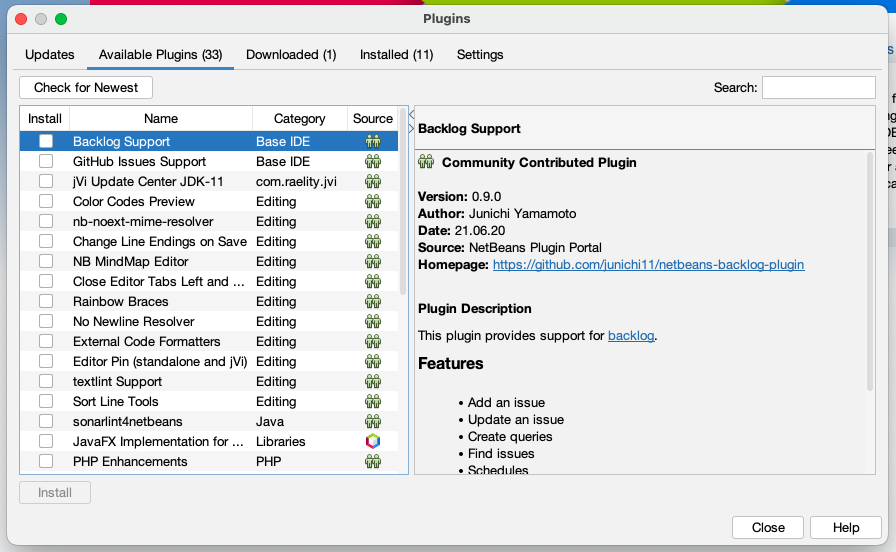
\includegraphics[width=0.8\textwidth]{obrazky-figures/plugin-portal/ide-pp.png}
	\caption{Funkce správy zásuvných modulů.}
	\label{pluginPortalVIDE}
\end{figure}

\subsubsection{Použití zásuvného modulu vytvořeného třetí stranou}
Existuje mnoho zásuvných modulů, které se v~oficiálním repozitáři nenachází. Pro instalaci takového modulu potřebujeme mít soubor s~příponou \texttt{NBM} určenou pro verzi použitého vývojového prostředí. Instalaci je pak možné provést pomocí funkce správy zásuvných modulů. Dále je možné instalovat moduly \emph{OSGi}~\cite{OSGi} s~příponou \texttt{JAR}.

\subsubsection{Vytvoření vlastního zásuvného modulu}
K~tvorbě vlastního zásuvného modulu lze využít již existující aplikační programové rozhraní \emph{Apache NetBeans}. Takový modul lze pak následně volně sdílet či zveřejnit na~\emph{Apache NetBeans Plugin Portalu}.

\section{Dostupné aplikační programové rozhraní}
Aplikační programové rozhraní ve vývojovém prostředí \emph{Apache NetBeans} poskytuje způsob, jakým lze vytvářet jazykové klienta~za~použití jazyku \emph{Java}. Aplikační programové rozhraní je implementováno za~použití knihovny \emph{LSP4J}~\cite{EclipseLSP4J}. \emph{LSP4J} je open-source knihovna~poskytující implementaci protokolu \emph{LSP} pro integrovaná vývojová prostředí psaná jazykem~\emph{Java}, jako je například \emph{Eclipse} nebo \emph{Apache NetBeans}. Knihovna~podporuje všechny funkce protokolu \emph{LSP}. Knihovna~je distribuovaná pod licencí \emph{Eclipse Public Licence 2.0}\footnote{Je zdarma~k~užití a~může být upravována~dle potřeb.}. Správa knihovny je v~režii aktivní komunity, která poskytuje nová vylepšení a~aktualizace. 

Implementovaný klient k~navázání spojení využívá třídu \texttt{LanguageServerProvider} modulu \texttt{org.netbeans.modules.lsp.client.spi}. Pro práci s~editorem kódu je k~dispozici modul \texttt{org.netbeans.api.editor}, který obsahuje i metody podstatné pro inicializaci jazykového klienta při otevření podporovaného souboru -- \texttt{MimeRegistration} a \texttt{MimeRegistrations}. Pro zpracování uživatelských preferencí je třeba implementovat vlastní třídu.

\section{Alternativní dostupná řešení}
\label{alternativniDostupnaReseni}
Vývojové prostředí \emph{Apache NetBeans} disponuje vestavěným jazykovým klientem s~možností omezené konfigurace vlastního jazykového serveru. Při použití vestavěného klienta ale nelze specifikovat potřebné parametry spuštění jazykového serveru. Důsledkem toho není vestavěný klient s~jazykovým serverem \emph{Apache Camel} vytvořeným společností \emph{Red Hat} kompatibilní. Přímé alternativní řešení tedy neexistuje. Vestavěného jazykového klienta lze použít dvěma způsoby popsanými níže.

\subsection{Registrace vlastního jazykového serveru}
Registrace vlastního jazykového serveru je možná po vyvolání průvodce nacházejícího se v~\texttt{Options → Editor → Language Servers}. Průvodce umožňuje specifikovat přípony, pro které se má jazykový server spouštět. Kromě samotného jazykového serveru lze připojit soubor se syntaktickou gramatikou\footnote{Určuje pravidla, podle kterých jsou zapisovány programové konstrukce a výrazy v~daném jazyce.}. Není možné ovšem specifikovat konkrétní instrukce pro spuštění jazykového serveru (jazykový server pro \emph{Apache Camel} vytvořený společností \emph{Red Hat} se spouští pomocí příkazu \texttt{java -jar}). Ke spuštění jazykového serveru tedy nedojde. Manuální spuštění jazykového serveru s~následným propojením není možné.

\subsection{Propojení s~jazykovým serverem}
Druhým způsobem, jak lze vestavěného jazykového klienta~propojit s~vývojovým prostředím \emph{Apache NetBeans}, je propojení pomocí \texttt{Connect to Language Server} z~nabídky \texttt{Tools}. Tato možnost vyžaduje již spuštěný jazykový server komunikující na~definovaném\footnote{Číslo portu může být libovolné.} síťovém portu. Jazykový server \emph{Apache Camel} vytvořený společností \emph{Red Hat} touto možností nedisponuje. Pro případné propojení lze vytvořit prostředníka, který bude přesměrovávat vstupní a~výstupní toky z~běžícího jazykového serveru na~síťový port. Takové řešení je uživatelsky velmi nepřívětivé. Implementace funkčních vlastností nad rámec povinného základu je nemožná. 

\chapter{Návrh jazykového klienta~pro Apache Camel}
\label{navrhJazykovehoKlienta}
Návrh klienta~je stěžejní součástí při procesu tvorby klientské aplikace. Kapitola~se věnuje popisu klíčových prvků při návrhu samotného modulu včetně podporovaných funkčních vlastností vytvářeného jazykového klienta. Dále kapitola~popisuje návrh uživatelského rozhraní. 

\section{Návrh architektury}
\label{navrhJazykovehoKlienta-navrhArchitektury}
Architektura zásuvného modulu se skládá ze dvou částí. První částí je samotná klientská aplikace pro jazykový server \emph{Apache Camel}. Ta zajišťuje komunikaci mezi integrovaným vývojovým prostředím a jazykovým serverem \emph{Apache Camel}. Druhou částí je samotný zásuvný modul pro vývojové prostředí. Zásuvný modul integruje vytvořenou klientskou aplikaci přímo do vývojového prostředí. Zároveň přidává uživatelské rozhraní pro správu a~nastavení modulu. 

Diagram~\ref{diagramkomunikacenavrhklienta} zobrazuje návrh architektury. Integrované vývojové prostředí (\emph{IDE}) \emph{Apache NetBeans} reprezentuje rozhraní pro editaci kódu. Uživatel otevře podporovaný soubor (libovolné \emph{Camel DSL\footnote{Doménově specifický jazyk (Domain Specific Language), viz kapitola~\ref{camelVlastnosti}.}}) uvnitř vývojového prostředí. Vývojové prostředí pomocí aplikační programového rozhraní (\emph{API}) nejprve spustí instanci jazykového klienta, následně s~ním za použití stejného rozhraní komunikuje. Jazykový klient naváže spojení s~jazykovým serverem \emph{Apache Camel}. Instance jazykového serveru je spuštěna jazykovým klientem po otevření podporovaného souboru, zásah uživatele není vyžadovaný. Jazykový klient a jazykový server spolu komunikují za užití \emph{Language Server Protokolu} popsaného v~kapitole~\ref{lsp}.

\begin{figure}[hbt]
	\centering
        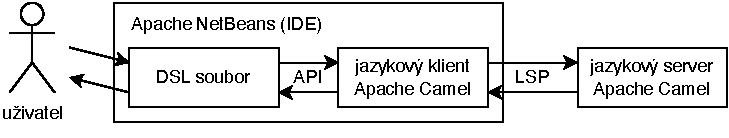
\includegraphics[width=1\columnwidth]{obrazky-figures/pdf/DiagramNavrh.pdf}
	\caption{Diagram zobrazující návrh architektury jazykového klienta.}
	\label{diagramkomunikacenavrhklienta}
\end{figure}

\section{Vlastnosti zásuvného modulu}
\label{navrhJazykovehoKlienta-vlastnostiModulu}
Jazykový klient byl navržen a~implementován tak, aby využil veškerý potenciál funkcí, které jazykový server vytvořený společností \emph{Red Hat} pro \emph{Apache Camel} nabízí. Mezi funkcionality jazykového serveru patří: 

\begin{itemize}
    \item \textbf{Dokončování kódu pro jednotné identifikátory zdroje (\emph{URI}) \emph{Camel}} -- Vývojové prostředí automaticky napovídá a dokončuje dostupné \emph{Camel} komponenty, atributy komponent a jejich hodnoty na základě dotazů odesílaných na server.
    \item \textbf{Diagnostika~a~validace jednotných identifikátorů zdroje \emph{Camel}} -- Vývojové prostředí automaticky zasílá požadavek na server, který kontroluje, zda jsou vložené \emph{Camel} komponenty, atributy komponent a jejich hodnoty validní.
    \item \textbf{Volba specifické verze katalogu komponent \emph{Camel}} -- Uživatel může specifikovat, jakou verzi katalogu komponent \emph{Camel} má jazykový server použít.
    \item \textbf{Volba specifického poskytovatele běhového prostředí katalogu komponent  \emph{Camel}} -- Uživatel může specifikovat, jakého poskytovatele běhového prostředí katalogu komponent \emph{Camel} má jazykový server použít.
    \item \textbf{Přidání vlastních komponent \emph{Camel}} -- Uživatel může rozšířit katalog komponent o~vlastní komponenty \emph{Camel}.
    \item \textbf{Propojení pro dokončování komponent \emph{Apache Kafka}} -- Uživatel může specifikovat adresu běžící instance \emph{Apache Kafka}, ze které jazykový klient přebírá informace o~běžících topicích, které následně nabízí při automatickém dokončování kódu.
    \item \textbf{Použití specifického jazykového serveru} -- Uživatel může specifikovat vlastní cestu k~jazykovému serveru, který je použitý. Není-li vlastní cesta specifikovaná, jazykový klient automaticky inicializuje poslední dostupnou verzi jazykového serveru bez nutnosti zásahu uživatele.
\end{itemize}

Všechny funkce jsou podporovány pro doménově specifické jazyky \emph{Java}, \emph{XML} a~\emph{YAML}. 

\section{Uživatelské rozhraní}
\label{navrhJazykovehoKlienta-uzivatelskeRozhrani}
Samotný jazykový klient využívá výchozího uživatelského rozhraní \emph{Apache NetBeans}. Pro cílového uživatele je nenápadný a~poskytuje mu implicitní podporu. Návrh uživatelského rozhraní se tedy omezuje pouze pro nastavení klienta. 

Při návrhu rozhraní bylo prioritou zachování intuitivnosti. V~rámci vývojového prostředí lze za~použití vhodného aplikačního rozhraní umístit nastavení na~libovolné místo. Za~nejvhodnější umístění je považováno přímo hlavní nastavení editoru. Pro modul bylo zvoleno nastavení v~samostatné záložce, oddělené od předinstalovaných jazykových klientů. Vzhled uživatelského rozhraní zobrazuje obrázek~\ref{navrhJazykovehoKlienta-nastaveniKlienta-img}. Samotné nastavení jazykového klienta~je intuitivní a~především nepovinné. Každý z~atributů má své výchozí hodnoty. 
\newpage
Uživatel si může nastavit následující: 
\begin{itemize}
    \item \textbf{Verze katalogu s~komponentami \emph{Camel}} -- Výchozí verzi stanovuje jazykový server, klient v~takovém případě odesílá hodnotu \texttt{DEFAULT}.
    \item \textbf{Poskytovatel běhového prostředí katalogu komponent \emph{Camel}} -- Výchozí hodnotu definuje jazykový server, klient odesílá hodnotu \texttt{DEFAULT}. Uživatel má na~výběr mezi \emph{Spring Boot}, \emph{Karaf} a~\emph{Quarkus}.
    \item \textbf{Přidání vlastní komponenty \emph{Camel}} -- Komponenty jsou vkládány jako validní \emph{JSON} list.\footnote{\url{https://camel.apache.org/manual/writing-components.html}} Výchozí hodnota~je \texttt{null}. Příklad viz výpis~\ref{lst:vlastnikomponenta}. 
    \item \textbf{Adresu pro propojení s~běžící instancí \emph{Apache Kafka}} --  Výchozí hodnota~je \texttt{localhost:9092}, což je výchozí adresa~\emph{Apache Kafka}. Jazykový klient tedy hledá běžící instance i bez nutnosti zásahu uživatele.
    \item \textbf{Vlastní jazykový server} -- Při zobrazení pokročilých možností si může uživatel definovat cestu k~vlastnímu jazykovému serveru \emph{Apache Camel}. Klient ve výchozím nastavení používá verzi \texttt{1.9.1}.
\end{itemize}

\begin{figure}[hbt]
	\centering
	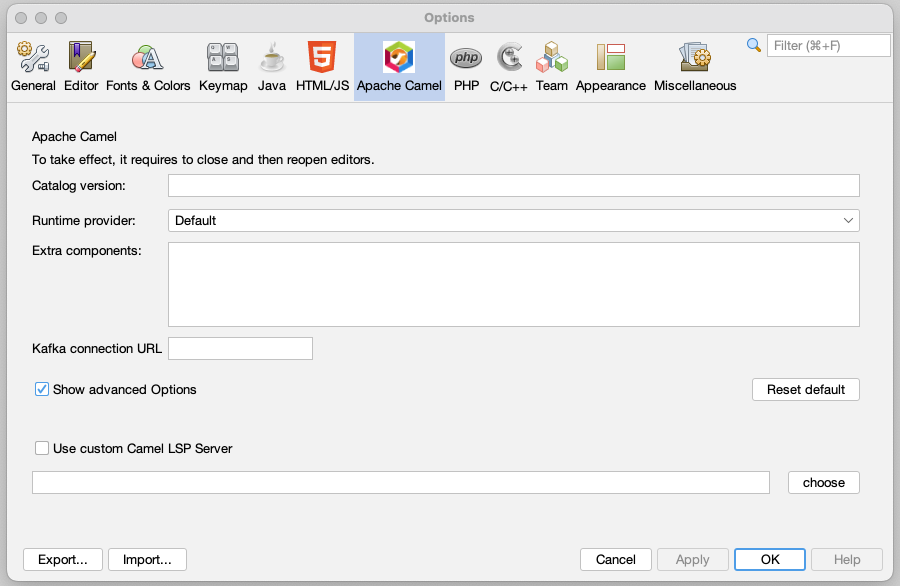
\includegraphics[width=\textwidth]{obrazky-figures/ui/options.png}
	\caption{Možnosti nastavení jazykového klienta.}
	\label{navrhJazykovehoKlienta-nastaveniKlienta-img}
\end{figure}

\chapter{Implementace zásuvného modulu}
\label{implementaceKlienta}
Na~základě vytvořeného návrhu jazykového klienta~je možné vytvořit zásuvný modul s~klientskou aplikací implementující jazykového klienta~pro \emph{Apache Camel}. Proces implementace lze rozdělit do několika~fází, které tato kapitola~popisuje. Kapitola~dále popisuje i nalezený nedostatek v~aplikačním programovém rozhraní a~návrh jeho řešení. 

\section{Postup vytváření jazykového klienta}

\subsubsection{Prerekvizity}
\label{implementaceKlienta-prerekvizity}
Pro vytvoření nového jazykového klienta~pro \emph{Apache NetBeans} je zapotřebí připravit lokální prostředí a~mít k~dispozici vývojové prostředí \emph{Apache NetBeans}, manažer balíčků \emph{Apache Maven}~\cite{maven} a jazykový server včetně nezbytných informací pro jeho spuštění. Dále je vhodné mít k~dispozici verzovací nástroj \emph{Git}~\cite{gitcite}.

\subsubsection{Založení nového projektu}
Prvním krokem pro vytvoření jazykového klienta~je založení nového projektu. Pomocí \texttt{File → New Project...} lze vyvolat průvodce pro založení projektu. Vývojové prostředí disponuje předdefinovanou šablonou pro tvorbu zásuvných modulů. Využívá k~tomu manažera~balíčku \emph{Apache Maven}.

Možností nastavení projektu jsou triviální a~lze je později změnit. Implementovaný jazykový klient je tvořen s~využitím verze \emph{Apache NetBeans 17.0}, která odpovídá označení \texttt{RELEASE170}.

\subsubsection{Konfigurace založeného projektu}
Samotné založení projektu pro tvorbu zásuvného modulu žádným způsobem nedefinuje jeho předurčení. Tvořený jazykový klient by měl být spouštěn pouze na~vyžádání. Tedy v~situacích, kdy je v~editoru aktivně otevřený soubor, kterému náš server poskytuje jazykovou podporu. Na~existujícím projektu lze pomocí předdefinované šablony takovou funkci vytvořit. Vyvoláním nabídky nad projektem \texttt{New → Other → Module Development → File Type} dojde k~otevření průvodce pro automatické rozpoznávání typů souborů.

Nastavení je třeba~věnovat zvýšenou pozornost, jeho pozdější změna~je obtížná. K~identifikaci typu souboru je využíván standard MIME~\cite{MozillaMIME}. Ten se skládá ze dvou částí -- typu a~podtypu. Tyto části jsou oddělené lomítkem. Pro tvořeného jazykového klienta~používáme typ \texttt{text}. Jazykový server \emph{Apache Camel} pracuje celkem se~třemi podtypy -- \emph{XML}, \emph{Java} a~\emph{YAML}. Jazykový klient tedy bude rozpoznávat následující definice: 
\begin{itemize}
    \item \texttt{text/xml},
    \item \texttt{text/java},
    \item \texttt{text/yaml}.
\end{itemize} 

Dále je třeba~definovat, zda požadovaný typ souboru má specifickou příponu nebo je tvořen kořenovým elementem \emph{XML}. Tvořený jazykový klient pro \emph{Apache Camel} bude rozpoznávat přípony \texttt{xml}, \texttt{java} a~\texttt{yaml}.

Po ukončení průvodce bude projekt obsahovat nové soubory. Kromě rozpoznání typu souboru lze tímto způsobem také do vývojového prostředí přidat zcela~nový typ souboru. Soubor \texttt{xmlTemplate.xml} obsahuje šablonu, která by se vložila~do nově vytvořeného souboru s~daným typem. Soubor \texttt{package-info.java} obsahuje informace spojené právě s~vložením této šablony. Protože v~rámci implementace jazykového klienta~šablony použity nebudou, nejsou tyto soubory relevantní a~z~projektu mohou být odstraněny. Stejný postup je třeba opakovat pro typy souborů \texttt{java} a~\texttt{yaml}. 

\subsubsection{Třída~s~jazykovým klientem}
Rozpoznávání typu souborů je nezbytnou součástí implementace jazykového klienta, samo o~sobě ale nepřináší žádnou funkcionalitu. Aby bylo možné klienta~implementovat, je třeba vytvořit novou třídu v~projektu. Třídu je možné pojmenovat zcela~libovolně. 

Nově vytvořená třída~bude implementovat \texttt{LanguageServerProvider} z~aplikačního programového rozhraní knihoven \emph{Apache NetBeans}. Třídu je třeba~importovat. Dále je třeba~importovat funkci \texttt{MimeRegistration} z~programového rozhraní editoru \emph{Apache NetBeans}. 

\texttt{MimeRegistration} zajišťuje stěžejní část nově vznikajícího klienta. Propojí integrované vývojové prostředí s~jazykovým klientem ve vhodnou chvíli. Konkrétně v~situaci, kdy je otevřen konkrétní soubor využívající definovaný \emph{MIME}. Jazykový klient pro \emph{Apache Camel} pracuje s~třemi různými doménově specifickými jazyky. Takovou situaci je možné řešit dvěma způsoby. Pro každý doménově specifický jazyk mohu vytvořit samostatnou třídu nebo mohu využít třídu \texttt{MimeRegistrations}, která mi umožní zaštítit jednu třídu s~jazykovým klientem více typy \emph{MIME}.

\subsubsection{Tvorba uživatelského rozhraní}
Integrované vývojové prostředí \emph{Apache NetBeans} využívá k~tvorbě grafického prostředí nástrojovou sadu \emph{Swing UI}. Příkladem užití ve vývojovém prostředí je například editor kódu, kde sada \emph{Swing UI} zajišťuje zvýrazňování syntaxe. Vývojové prostředí \emph{Apache NetBeans} obsahuje základní šablony pro tvorbu uživatelských rozhraní, které je možné použít.

Na existujícím projektu lze vyvolat průvodce pro využití šablon pomocí \texttt{New → Other → Module Development}. K~dispozici je více druhů šablon. Pro implementaci uživatelského nastavení přímo v~rozhraní vývojového prostředí je vhodná pouze šablona \texttt{Options Panel}. Průvodce je velmi intuitivní a jeho nastavení je snadné. Nastavení jazykového klienta pro Apache Camel je implementováno jako primární panel, tedy nastavení je zcela oddělené na samostatné záložce. Průvodce vygeneruje soubory \texttt{Panel.form}, \texttt{Panel.java}, \texttt{OptionsPanelController.java}.

\texttt{Panel.form} a \texttt{Panel.java} reprezentují grafické rozhraní modulu. \texttt{Panel.java} lze ote\-vřít pomocí grafického editoru \texttt{Design}. Uvnitř grafického editoru lze snadno navrhovat uživatelské rozhraní. Soubor \texttt{Panel.form} je generován automaticky a není nutné do něj zasahovat. \texttt{OptionsPanelController.java} představuje třídu sdružující veškeré operace vykonané nad vytvořeným uživatelským rozhraním. Veškerá implementace spojená se tvorbou a~zpracováním uživatelských preferencí se nachází zde.

\section{Problém a~jeho řešení}
Přítomnost uživatelského nastavení je stěžejní přidanou hodnotou dedikovaného jazykového klienta. K~předávání spouštěcích parametrů klienta~dochází ihned po spuštění jazykového serveru. Parametry jsou předávány ve formátu \emph{JSON-RPC} během první zprávy směřované na~jazykový server. Složení první zprávy zobrazuje obrázek~\ref{slozeniPrvniZpravyNaServer}. V~průběhu implementace těchto přidaných funkcionalit bylo nalezeno nedostatečné pokrytí ze strany aplikačního programového rozhraní \emph{Apache NetBeans}. Po kompletním přezkoumání dokumentace i zdrojových kódu byl utvořen závěr, že tyto parametry se současnou implementací aplikačního rozhraní nelze serveru předat. Na~dané téma~byla~otevřena~v~komunitě \emph{Apache NetBeans} diskuze\footnote{\url{https://github.com/apache/netbeans/discussions/5776}}, která i po měsíci zůstala~bez odpovědi.

Aplikační programové rozhraní \emph{Apache NetBeans} využívá knihovnu \emph{LSP4J}. Knihovna \emph{LSP4J} poskytuje základní implementaci nízkoúrovňového aplikačního rozhraní \emph{Language Server Protocolu} pro prostředí využívající jazyk \emph{Java}. Implementace této knihovny obsahuje i funkci \texttt{setInitializationOptions}, která zajišťuje předání inicializačních parametrů jazykovému serveru. Pro zachování objektivnosti je třeba~zmínit, že tyto parametry nejsou povinné a~komunikaci lze úspěšně zahájit i bez jejich přítomnosti.\footnote{Funkce jsou v~takovém případě omezené na povinné minimum.} I~přes to danou absenci považuji za~hrubý nedostatek. Na~základě daného zjištění jsem založil nový požadavek na~rozšíření aplikačního rozhraní,\footnote{\url{https://github.com/apache/netbeans/issues/5822}} včetně návrhu mého řešení, které je popsáno v~následujících odstavcích. 

\begin{figure}[hbt]
	\centering
        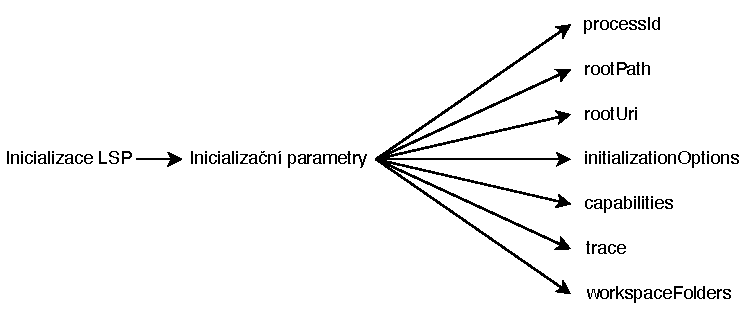
\includegraphics[width=0.8\columnwidth]{obrazky-figures/pdf/inicializace.pdf}
	\caption{Složení první zprávy odesílané na server.}
	\label{slozeniPrvniZpravyNaServer}
\end{figure}

\subsubsection{Analýza~problému}
Pro možnost navržení alternativního řešení bylo nezbytné nejprve dostatečně pochopit způsob, jakým aplikační rozhraní \emph{Apache NetBeans} pracuje s~nízkoúrovňovou knihovnou \emph{LSP4J}. 

Komunikace probíhá následovně: 
\begin{enumerate}
    \item Při vytvoření nové instance jazykového klienta~je volán konstruktor \texttt{LanguageServerDescription}. Konstruktor je součástí třídy \texttt{LanguageServerProvider} a~akceptuje tři parametry -- tok vstupních dat, tok výstupních dat a~proces jazykového serveru. 
    \item Třída~\texttt{LanguageServerProvider} při své inicializaci využívá třídy \texttt{LSPBindings}, která zajišťuje vazbu mezi jazykovým klientem a~jazykovým serverem. První volanou metodou je metoda~\texttt{getBindings}, která zajišťuje získání potřebných vazeb. Implementována~je ve funkci \texttt{getBindingsImpl}. Ta~volá metodu \texttt{buildBindings}, která vytváří vazbu mezi klientem a~jazykovým serverem. 
    \item K~předání parametrů pro inicializaci serveru dochází pomocí metody \texttt{initServer}, která je inicializována~v~průběhu metody \texttt{buildBindings}. V~této části také chybí možnost přidání vlastních parametrů typu \texttt{initializationOptions}. 
    \item Jazykový server je spuštěn s~předanými parametry. 
\end{enumerate}

\subsubsection{Řešení}
Stěžejní problém je tvořen skutečností, že nelze při inicializaci jazykového serveru metodou \texttt{initServer} předat vlastní parametry. Konstruktor dané metody jsem tedy rozšířil o~další parametr \texttt{initOptions}. Parametr je typu \texttt{Object}, přijímá tedy libovolný objekt. 
\begin{lstlisting}[language=JAVA, label={lst:implementaceKlienta-reseni-kod-1}, caption=Konstruktor funkce \texttt{initServer} s~přidaným parametrem.]
private static InitializeResult initServer(Process p, LanguageServer server, FileObject root, Object initOptions);
\end{lstlisting}
Nově přidaný parametr je uvnitř funkce \texttt{initServer} zpracován pouze je-li jeho hodnota odlišná od \texttt{null}, v~opačném případě není hodnota~\texttt{setInitializationOptions} inicializována.

\begin{lstlisting}[language=JAVA, label={lst:implementaceKlienta-reseni-kod-2}, caption=Zpracování parametru \texttt{initOptions}.]
private static InitializeResult initServer(...) {
    InitializeParams initParams = new InitializeParams();
    ...
    if(initOptions != null){
        initParams.setInitializationOptions(initOptions);
    }
    ...
}
\end{lstlisting}
Metoda~\texttt{initServer} je volána~z~metod \texttt{buildBindings} a~\texttt{addBindings}. Druhá zmíněná metoda~není pro rozšíření prostředí podstatná, pro zachování funkčnosti je pouze třeba~doplnit čtvrtý parametr s~hodnotou \texttt{null}. 
\begin{lstlisting}[language=JAVA, label={lst:implementaceKlienta-reseni-kod-3}, caption=Rozšíření metody \texttt{addBindings}.]
public static void addBindings(..){
...
InitializeResult result = initServer(null, server, root, null);
...
}
\end{lstlisting}
Metoda~\texttt{buildBindings} je pro řešení podstatná. Tato~metoda~přebírá hodnoty z~\texttt{LanguageServerProviderAccessor}, který zajišťuje instanci jazykového serveru. Tuto třídu bude také nezbytné upravit. 
\begin{lstlisting}[language=JAVA, label={lst:implementaceKlienta-reseni-kod-4}, caption=Rozšíření metody \texttt{buildBindings}.]
private static LSPBindings buildBindings(...) {
...
try {
    ...
    Object initOpt = LanguageServerProviderAccessor.getINSTANCE().getInitOptions(desc);
    ...
    InitializeResult result = initServer(p, server, dir, initOpt);
    ...
}
... 
}
\end{lstlisting}
Třídu \texttt{LanguageServerProviderAccessor} zajišťující běh instance jazykového serveru rozšířím o~abstraktní metody pro nastavení a~získání hodnot inicializačních hodnot.
\begin{lstlisting}[language=JAVA, label={lst:implementaceKlienta-reseni-kod-5}, caption=Rozšíření třídy \texttt{LanguageServerProviderAccessor}.]
public abstract class LanguageServerProviderAccessor {
...
    public abstract Object getInitOptions(LanguageServerDescription desc);    
    public abstract void setInitOptions(LanguageServerDescription desc, Object initOptions);  
}
\end{lstlisting}
Samotnou implementaci abstraktních metod provádím v~rozhraní \texttt{LanguageServerProvider} a~třídě \texttt{LanguageServerDescription}. Rozhraní je třeba~rozšířit hned o~několik vlastností. Je nutné založit privátní proměnnou zajišťující Objekt \texttt{initOptions}. Dále je potřeba~přidat nový konstruktor pro vytvoření instance jazykového klienta~přijímající parametr \texttt{initOptions}. Po rozšíření o~nový konstruktor je třeba~ošetřit zachování zpětné kompatibility při volání původního konstruktoru.

\begin{lstlisting}[language=JAVA, label={lst:implementaceKlienta-reseni-kod-6}, caption=Rozšíření třídy \texttt{LanguageServerDescription} o~druhý konstruktor.]
public interface LanguageServerProvider {
...
    public static final class LanguageServerDescription {
        public static @NonNull LanguageServerDescription create(@NonNull InputStream in, @NonNull OutputStream out, @NullAllowed Process process) {
            return new LanguageServerDescription(in, out, process, null);
        }
        public static @NonNull LanguageServerDescription create(@NonNull InputStream in, @NonNull OutputStream out, @NullAllowed Process process, @NullAllowed Object initOptions) {
            return new LanguageServerDescription(in, out, process, initOptions);
        }
...
}
\end{lstlisting}
Oba~konstruktory při předávání své návratové hodnoty vracejí novou instanci \texttt{LanguageServerDescription}. Konstruktor s~třemi parametry na~místo očekávaného nového parametru dosazuje hodnotu \texttt{null}. Tím je zachována~zpětná kompatibilita~při volání původního konstruktoru.
\begin{lstlisting}[language=JAVA, label={lst:implementaceKlienta-reseni-kod-7}, caption=Zpracování nových parametrů třídou \texttt{LanguageServerDescription}.]
public interface LanguageServerProvider {
...
    public static final class LanguageServerDescription {
        ...
        private Object initOptions;
        ...
        private LanguageServerDescription(InputStream in, OutputStream out, Process process, Object initOptions) {
                ...
                this.initOptions = initOptions;
            }
        }
        ...
    }
}
\end{lstlisting}

Takto upravené aplikační rozhraní je potřeba~zkompletovat pomocí nástroje \texttt{ant}~\cite{ApacheANT}. Nově vzniklý soubor s~upraveným aplikačním rozhraním je nutné připojit jako závislost do implementace jazykového klienta. Zdrojové kódy k~upravenému aplikačnímu rozhraní jsou součástí přílohy této bakalářské práce.

\section{Publikace zásuvného modulu}
Zásuvný modul vytvořený v~této práci je v~plánu publikovat v~repozitáři zásuvných modulů \emph{Apache NetBeans Plugin Portal}. To nyní není na základě nutné úpravy aplikačního programového rozhraní pro zajištění kompletní funkčnosti jazykového klienta~možné. Po rozšíření aplikačního rozhraní o~funkci inicializace parametrů bude možné jazykového klienta~přizpůsobit a~následně zveřejnit. 
Zásuvný modul bude procházet posouzením ověřených dobrovolníků z~komunity \emph{Apache NetBeans}. Po jejich schválení bude zásuvný modul publikován. 

\chapter{Ověření funkcionality}
\label{overeniFunkcnosti}
Nedílnou součástí procesu vývoje aplikací je testování. Automatizace testování na~úrovni uživatelského rozhraní je obtížná, při absenci vhodného integračního rozhraní až nemožná. Proto bylo zvoleno manuální testování na základě testovacích scénářů. Tato kapitola~popisuje testovací scénáře pro jednotlivé funkční vlastnosti jazykového klienta. Součástí jsou i~jednotlivé kroky pro manuální testování.

\section{Testování jazykového klienta}
Pro ověření funkčnosti klienta~slouží následující manuální testovací
scénáře. Pro testování je třeba použít instanci \emph{Apache NetBeans} obsahující upravené aplikační programové rozhraní. Spuštění je popsáno v~manuálu obsaženém v~příloze této bakalářské práce. Pro testování je možné použít následující kód. Po každé změně v~nastavení klienta~je třeba~restartovat vývojové prostředí, aby se změny projevily.
    \begin{lstlisting}[language=XML, label={lst:camelrouteexamplekod}, caption=Kód použitý v~testovacích scénářích.]
<?xml version="1.0" encoding="UTF-8"?>
<camelContext id="cbr-example-context"
xmlns="http://camel.apache.org/schema/spring">
    <route id="cbr-route">
        <from id="_from1" uri=""/>
    </route>
</camelContext>
    \end{lstlisting}

\subsection{Přítomnost klienta~ve vývojovém prostředí}
Cílem testovacího scénáře je ověřit, že je klient ve vývojovém prostředí \emph{Apache NetBeans} nainstalován a~je aktivní.
\begin{enumerate}
    \item Z~nabídky rozhraní prostředí \emph{Apache NetBeans} otevřít menu \texttt{Tools}.
    \item V~nabídce \texttt{Tools} zvolit vnořenou položku \texttt{Plugins}.
    \item Otevřít záložku \texttt{Installed} a~ověřit, že zásuvný modul je nainstalován a~je aktivní, viz obrázek~\ref{testovani-pritomnost-img}.
\end{enumerate}

\begin{figure}[hbt]
	\centering
	
\includegraphics[width=\textwidth]{obrazky-figures/tests/pritomnostVIDE/1.png}
	\caption{Nainstalovaný a~aktivní zásuvný modul s~klientem.}
	\label{testovani-pritomnost-img}
\end{figure}

\subsection{Dokončování kódu}
Testovací scénář ověřuje základní funkční vlastnost v~podobě automatického dokončování kódu včetně doplňování atributů a~jejich hodnot.

\begin{enumerate}
    \item V~libovolném projektu vytvořit soubor pojmenovaný například \texttt{camel-route.xml}.
    \item Jako obsah souboru vložit kód z~výpisu~\ref{lst:camelrouteexamplekod}.
    \item Umístit kurzor mezi uvozovky na~5. řádku u~atributu \texttt{uri} a~vyvolat kontextovou nabídku použitím klávesové zkratky \texttt{Control + mezera}. Viz obrázek~\ref{testovani-dokoncovani-img}.
    \begin{figure}[hbt]
	\centering
	
\includegraphics[width=\textwidth]{obrazky-figures/tests/dokoncovani/1.png}
	\caption{Kontextová nabídka~zobrazující dostupné komponenty.}
	\label{testovani-dokoncovani-img}
    \end{figure}
    \item Z~nabídky vybrat komponentu \texttt{timer:timerName}.
    \item Doplnit za~komponentu znak \texttt{?} a~vyvolat kontextovou nabídku, jestliže se nevyvolala~automaticky.
    \item Ze seznamu atributů vybrat \texttt{delay}.
    \item Ověřit, že došlo k~doplnění výchozí hodnoty \texttt{'=1000'} a~řádek obsahující komponentu vypadá následovně:
    \begin{lstlisting}[language=XML]
<from id="_from1" uri="timer:timerName?delay=1000"/>
    \end{lstlisting}
\end{enumerate}


\subsection{Diagnostika~a~validace}
Testovací scénář ověřuje dostupnost diagnostiky a~validace atributů u~komponent. Vývojové prostředí automaticky zasílá požadavek na server, který kontroluje, zda jsou vložené \emph{Camel} komponenty, atributy komponent a jejich hodnoty validní\footnote{Komponenta a její atributy existují. Hodnoty atributů mají platný datový typ a formát.}.
\begin{enumerate}
    \item Opakovat postup testování dokončování kódu.
    \item Za~hodnotu \texttt{'delay=1000'} doplnit znak \texttt{r}, řádek tedy dostane tvar:
    \begin{lstlisting}[language=XML]
<from id="_from1" uri="timer:timerName?delay=1000r"/>
    \end{lstlisting}
    \item Zkontrolovat, že je řádek zvýrazněný a~klient hlásí diagnostickou chybu. Viz obrázek~\ref{testovani-diagnostika-chybnych-atributu-img}.
    \begin{figure}[hbt]
	\centering
	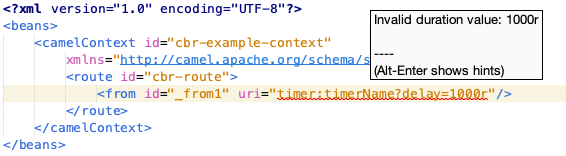
\includegraphics[width=0.9\textwidth]{obrazky-figures/tests/diagnostika/1.png}
	\caption{Diagnostika~chybných atributů komponenty.}
	\label{testovani-diagnostika-chybnych-atributu-img}
    \end{figure}
\end{enumerate}

\subsection{Použití specifické verze katalogu}
Testovací scénář ověřuje, že klient umí přepínat verze katalogů. Starší verze katalogů neobsahují stejné komponenty jako verze novější. Testovací scénář této skutečnosti využívá. Výchozí katalog ve verzi \texttt{2.15.1} neobsahuje komponentu \texttt{file-watch}. Při specifikování této konkrétní verze tedy komponenta~v~kontextové nabídce nemůže být dostupná.
\begin{enumerate}
    \item Nastavit verzi katalogu na~\texttt{2.15.1}.
    \item Mezi uvozovky na~5. řádku u~atributu \texttt{uri} vložit \texttt{file} a~vyvolat kontextovou nabídku.
    \item Zkontrolovat, že nabídka~neobsahuje komponentu \texttt{file-watch}.
    \item Změnit verzi katalogu zpět na~výchozí. 
    \item Opakovat krok 2.
    \item Ověřit, že s~výchozím katalogem je komponenta~\texttt{file-watch} v~kontextové nabídce dostupná.
\end{enumerate}

\subsection{Použití specifického poskytovatele běhového prostředí}
Testovací scénář ověřuje, že klient umí přepínat různé poskytovatele běhového prostředí. Různí poskytovatelé běhových prostředí neposkytují podporu pro všechny komponenty. Stejně tedy jako u~testování specifických verzí katalogů lze této skutečnosti využít pro ověření korektnosti nastavení. Katalog komponent běhového prostředí \texttt{Quarkus} neobsahuje komponentu \texttt{JMX}, při vyvolání kontextové nabídky tedy komponenta~nemůže být dostupná. Na~rozdíl od starší verze katalogu je ale nutné počítat se skutečností, že se jednotlivé katalogy o~komponenty stále rozšiřují, testovaná komponenta~tedy může být později dostupná a~testovací scénář bude vyžadovat změnu komponenty. Dostupnost komponent lze ověřit na~stránkách jednotlivých poskytovatelů běhových prostředí.

\begin{enumerate}
    \item Nastavit poskytovatele běhového prostředí na hodnotu \texttt{Quarkus}.
    \item Mezi uvozovky na~5. řádku u~atributu \texttt{uri} vložit \texttt{jmx} a~vyvolat kontextovou nabídku.
    \item Zkontrolovat, že nabídka~neobsahuje komponentu \texttt{jmx:serverURL}.
    \item Změnit poskytovatele běhového prostředí zpět na~výchozí. 
    \item Opakovat krok 2.
    \item Ověřit, že s~výchozím běhovým prostředím je komponenta~\texttt{jmx:serverURL} v~kontextové nabídce dostupná.
\end{enumerate}

\subsection{Přidání vlastních komponent}
Libovolný katalog komponent lze rozšířit o~nabízení vlastních komponent. Testovací scénář ověřuje, zda-li jsou vlastní komponenty k~dispozici v~kontextové nabídce jazykového klienta.
\begin{enumerate}
    \item V~nastavení vložit vlastní komponentu.
        \begin{lstlisting}[language=XML, label={lst:vlastnikomponenta}, caption=Kód vlastní komponenty.]
[
{
   "component":{
      "kind":"component",
      "scheme":"abcd",
      "syntax":"abcd:xyz"
   }
}
]
    \end{lstlisting}
    \item Mezi uvozovky na~6. řádku u~atributu \texttt{uri} vložit \texttt{abc} a~vyvolat kontextovou nabídku.
    \item Zkontrolovat, že nabídka~obsahuje komponentu \texttt{abcd:xyz}.

     \begin{figure}[hbt]
	\centering
	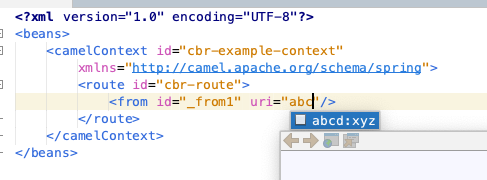
\includegraphics[width=120mm]{obrazky-figures/tests/extraKomponenty/ex1.png}
	\caption{Kontextová nabídka~obsahující vlastní komponentu.}
	\label{testovani-pridani-vlastnich-komponent-obsahuje-vlastni-komponentu-img}
    \end{figure}
\end{enumerate}

\subsection{Propojení pro dokončování komponent Apache Kafka}
Testovací scénář ověřuje dostupnost atributu obsahujícího název topiců běžící instance \emph{Apache Kafka} pro \emph{Camel} komponentu \texttt{kafka}. Prerekvizity: Běžící instance \emph{Apache Kafka} na adrese odlišné od \texttt{localhost:9092}. Tato adresa je výchozí a jazykový klient se s~ní pokouší navázat spojení bez nutnosti zásahu uživatele. Vhodná je například adresa \texttt{localhost:9093}. Instance \emph{Apache Kafka} již musí obsahovat alespoň jeden běžící topic, například \texttt{quickstart-events}.

\begin{enumerate}
    \item Nastavit adresu \emph{Apache Kafka} dle běžící instance, například na \texttt{localhost:9093}.
    \item Mezi uvozovky na~6. řádku u~atributu \texttt{uri} vložit \texttt{kafka:} a vyvolat kontextovou nabídku.
    \item Ověřit, že je k~dispozici atribut obsahující název topicu, například \texttt{quickstart-events}, viz obrázek~\ref{testovani-kafka-img}.
    \begin{figure}[hbt]
        \centering
            
\includegraphics[width=130mm]{obrazky-figures/tests/kafka/1.png}
        \caption{Doplnění atributu topicu Apache Kafka.}
        \label{testovani-kafka-img}
    \end{figure}\end{enumerate}


\subsection{Použití specifického jazykového serveru}
Pro případ, že by uživatel nechtěl použít výchozí jazykový server, může si zvolit cestu k~vlastnímu jazykovému serveru. Testovací scénář ověřuje, zda-li je použit specifikovaný jazykový server.
\begin{enumerate}
    \item V~nastavení aktivovat přepínač pokročilého nastavení (\texttt{Advanced options}). 
    \item Ze souborového systému vybrat cestu k~jinému jazykovému serveru \emph{Apache Camel}. 
    \item Otevřít soubor obsahující doménově specifický jazyk. 
    \item Pomocí nástroje \texttt{jps}~\cite{jps} ověřit, že se spustila požadovaná verze serveru.
    
    \begin{figure}[hbt]
        \centering
        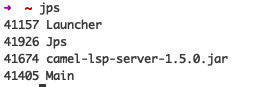
\includegraphics[width=70mm]{obrazky-figures/tests/vlastniLspServer/jps.png}
        \caption{Výpis nástroje jps.}
        \label{testovani-vypis-nastroje-jps-img}
    \end{figure}
\end{enumerate}

\section{Srovnání s~vestavěným jazykovým klientem}
Jak bylo uvedeno v~kapitole~\ref{alternativniDostupnaReseni}, vestavěný jazykový klient ve vývojovém prostředí \emph{Apache NetBeans} není možné pro jazykový server \emph{Apache Camel} použít. Srovnání tedy může probíhat pouze v~teoretické rovině a~za~předpokladu, že by nakonfigurovaný vestavěný jazykový klient byl s~jazykovým serverem \emph{Apache Camel} kompatibilní.

Největší výhodou vlastní implementace jazykového klienta~je uživatelská přívětivost. Instalace takového zásuvného modulu z~repozitáře zásuvných modulů \emph{Apache NetBeans Plugin Portal} či přímá instalace ze souboru se zásuvným modulem nevyžaduje žádnou dodatečnou konfiguraci a pro uživatele instalace obnáší jen pár kliknutí. Vestavěný jazykový klient takovou konfiguraci vyžaduje. Ze strany vývojového prostředí jsou navíc požadavky nejasné, konfigurace tedy není příliš přívětivá. 

Vestavěný jazykový klient by také uměl využít pouze určitou část funkčních vlastností jazykového klienta. Zcela~jistě by bylo možné provozovat základní funkční vlastnosti jako je dokončování komponent, atributů a~hodnot atributů. V~případě, že klient nepředává serveru žádné specifické požadavky, server pracuje se svými výchozími hodnotami. Podpora~pro typy souborů \texttt{xml}, \texttt{yaml} a~\texttt{java} by byla~zachována~i v~případě použití vestavěného klienta. Nebylo by tedy nutné vytvářet tři konfigurace. Vestavěný klient umožňuje specifikovat více něž jeden atribut definující typ souboru.

Vestavěný klient by neumožňoval využít přidanou hodnotu implementovaného klienta v~podobě pokročilých nastavení, která jsou dostupná z~uživatelského rozhraní a~popsaná v~kapitole~\ref{navrhJazykovehoKlienta-uzivatelskeRozhrani}. Nebylo by tedy možné použít jiné verze katalogu, jiné poskytovatele běhového prostředí či vlastní komponenty.

\chapter{Závěr}
\label{zaver}
Cílem bakalářské práce byl návrh zásuvného modulu poskytujícího jazykovou podporu pro rámec \emph{Apache Camel} v~integrovaném vývojovém prostředí \emph{Apache NetBeans} a~následná implementace navrženého zásuvného modulu postaveného nad aplikačním programovým rozhraním vývojového prostředí. 

V~rámci analýzy potřeb k~řešení zadání bakalářské práce bylo nejprve nutné se blíže seznámit s~jazykovým protokolem \emph{Language Server Protocol} a~s~jeho architekturou. Dále bylo zapotřebí nastudovat rámec \emph{Apache Camel} a~jeho již existující dostupnou implementaci jazykového serveru. V~poslední části teoretického seznámení bylo~nastudováno integrované vývojové prostředí \emph{Apache NetBeans}, možnosti jeho rozšíření a~aplikační programové rozhraní užívané k~vývoji zásuvných modulů. 

Základním předpokladem jazykového klienta~byla~uživatelská přívětivost. Při návrhu jazykového klienta~bylo zapotřebí nastudovat rámec \emph{Swing}, sloužící pro tvorbu grafických rozhraní v~prostředí \emph{Java}. Při návrhu architektury bylo také nezbytné specifikovat jednotlivé funkční vlastnosti tvořeného jazykového klienta.

Výstupem bakalářské práce je funkční jazykový klient. Zásuvný modul s~jazykovým klientem bylo zapotřebí implementovat na~základě návrhu, který byl vytvořen. Během implementace zásuvného modulu byl objeven zásadní nedostatek v~aplikačním programovém rozhraní integrovaného vývojového prostředí \emph{Apache NetBeans}. Na~základě této skutečnosti byl vypracován návrh řešení a otevřen požadavek na začlenění vlastnosti. Požadavek nyní čeká na vyřízení komunitou \emph{Apache NetBeans}. I~přes tuto skutečnost bylo možné jazykového klienta~implementovat v~plném rozsahu.

Po úspěšné implementaci jazykového klienta~byly provedeno testování. Pro proces testování byly navrženy manuální testovací scénáře, vycházející z~funkčních vlastností implementovaného klienta. Vytvořený klient byl také porovnán s~alternativními dostupnými řešeními. 

Všechny zadané cíle této práce byly úspěšně splněny, ověřeny a~výsledný jazykový klient vyplnil požadavky firmy \emph{Red Hat} pro použití v~praxi a budoucí vývoj klienta. Ten~je v~současné době limitován aplikačním rozhraním vývojového prostředí \emph{Apache NetBeans}. Po začlenění navrhovaných úprav do aplikačního programového rozhraní bude možné vzniklého klienta~publikovat v~repozitáři zásuvných modulů \emph{Apache NetBeans Plugin Portal}. Dále bude možné klienta~v~budoucnu rozšiřovat o~nové funkční vlastnosti, které jazykový server pro \emph{Apache Camel} plánuje poskytovat.